\documentclass{beamer}
% \documentclass[notes=only]{beamer}
\usepackage{tikz}
\usepackage{graphicx}
\graphicspath{{../resources/figures/}}
\usepackage{pgfpages}
\usepackage[style=nature,citestyle=numeric]{biblatex}
\usepackage[export]{adjustbox}
\usepackage{appendixnumberbeamer}
\usepackage{relsize}
% \usepackage[threecols]{hackthefootline}
\usepackage{tikzlings}
\usepackage{setspace}
\usepackage{ragged2e}
\usepackage[hang]{footmisc}
\usepackage{bm}
\usetikzlibrary{shapes,arrows,calc,positioning}
\usefonttheme{professionalfonts}
\usetheme{Boadilla}

\addbibresource{../resources/prospectus.bib}
\setbeamertemplate{navigation symbols}{}%remove navigation symbols
% \beamertemplatenavigationsymbolsempty
\hypersetup{pdfstartview={Fit}} % fits the presentation to the window when first displayed
% \emergencystretch=1em

% \setbeameroption{hide notes} % Only slides
% \setbeameroption{show only notes} % Only notes
% \setbeameroption{show notes on second screen=right} % Both

% Give a slight yellow tint to the notes page
% \setbeamertemplate{note page}{\pagecolor{yellow!5}\insertnote}\usepackage{palatino}

% \htfconfig{title=short, authinst=instpths, date=none, framenrs=fraction}
% \addtobeamertemplate{frametitle}{}{\vspace{-1em}} % decrease

\newcommand{\red}[1]{\textcolor{red}{#1}}
\newcommand{\green}[1]{\textcolor{green}{#1}}
\newcommand{\blue}[1]{\textcolor{blue}{#1}}
\newcommand*\pct{\scalebox{.9}{\%}}
\newcommand{\inlinefigure}[1]{%
  \begingroup\normalfont
  \includegraphics[height=\fontcharht\font`\B]{#1}%
  \endgroup
}

% Title information ------------------------------------------------------------
\title[Artifacts in Sequence Alignment]{Modeling artifacts in sequence alignment}
\vspace{2em}
\titlegraphic{%
\vspace{-2em}\includegraphics[width=0.3\linewidth,height=2cm]{images/biodesign_logo.png}%
\hspace{2.5cm}%
\includegraphics[width=0.35\linewidth,height=2cm]{images/fulton_logo.png}%
}
% \titlegraphic{\includegraphics[width=\textwidth,height=.5\textheight]{someimage}}
\author[JJ Garcia Mesa]{Juan J Garcia Mesa\\ \vspace{2em}
						{\small Reed Cartwright\\
						Banu Ozkan\\
						Jay Taylor\\
						Ted Pavlic}}
\date{}
% \titlegraphic{\includegraphics[width=.3\linewidth]{}}
%-------------------------------------------------------------------------------

\begin{document}
\maketitle

\begin{frame}{Personal Background} %---------------------------------------------------------
\begin{columns}
\column{0.7\textwidth}
\begin{itemize}
	\setlength\itemsep{1em}
	\item B.S. Computer Science, University of Barcelona, 2012-2014 (transfer)
	\item B.A. Interdisciplinary Studies (Sustainability \& Computational
		Mathematical Sciences), ASU, 2017
	\item Assistant Software Engineer, 2017-2018
	% \item \green{Software Carpentry Certified Instructor, 2018.}
	\item Biological Design PhD, ASU, 2018-
\end{itemize}
\column{0.3\textwidth}
\includegraphics[scale=0.075,center]{images/asu_fork.png}
\end{columns}
% \footnotetext[1]{\cite{mafft_katoh_2009}}  %% example for citing images
\end{frame} %-------------------------------------------------------------------

\begin{frame}{Sequence Alignment} %---------------------------------------------
% Importance of alignment
\begin{columns}
\column{0.5\textwidth}	
\begin{itemize}
	\setlength\itemsep{1em}
	\item Hypothesis of which characters are related by common descent \parencite{problems_cartwright_2009}.
	\item Sequence alignment is a fundamental task that precedes many genomic
			analyses \parencite{sequence_alignment_rosenberg_2009}.
	\item Often seen as an \textit{ad hoc} problem \cite{morrison_MSA_2018}.
\end{itemize}
\column{0.5\textwidth}	
\includegraphics[width=\textwidth,right]{images/pipeline.png}
\end{columns}
\note[item]{[...] such as phylogenetic inference, measurement of selection, gene
			annotation (among others).}
\end{frame} %-------------------------------------------------------------------

\begin{frame}{Artifacts in Genomic Data} %--------------------------------------
Uncorrected errors in genomic datasets can lead to inaccurate results in
functional and comparative genomic studies \parencite{estimates_schneider_2009}.
\begin{itemize}
	\item Frameshifts
	\item Early stop codons
	\item Within-codon indels
\end{itemize}
\vspace{1em}
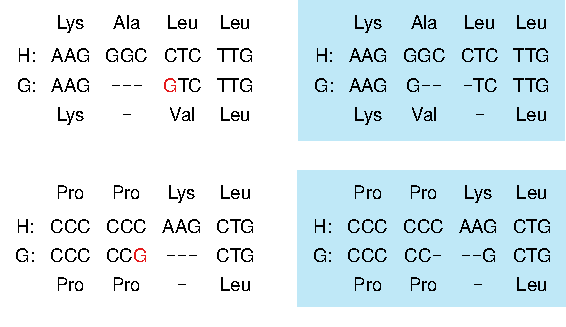
\includegraphics[scale=0.8,center]{fig-aln.pdf}

\note[item]{Current coding sequence aligners don't model correctly within codon
	gaps and frameshifts because generally alns are done based on amino acid
	translations.}
\note[item]{In data set used prelim results (4000 homologous human-gorilla pairs}
\note[item]{Avg across aligners: 1.07 frameshifts/locus, 0.28 stop codons/locus}
\note[item]{(in reality, 2340 were gapless, 2.59 frameshifts per locus)}
\end{frame} %-------------------------------------------------------------------
% models=(clustalo macse mafft mcoati prank)
% [jgarc111@hines CoatiAlign 16:11]$ for model in ${models[*]}; do bin/salsa sequence stop aln/${model}/*.fasta; done
% total count,7501  (clustalo)
% total count,166   (macse)
% total count,9012  (mafft)
% total count,491   (mcoati)
% total count,0     (prank)
% avg 4292 (no including prank)
% [jgarc111@hines CoatiAlign 16:11]$ for model in ${models[*]}; do bin/salsa gap frameshift aln/${model}/*.fasta; done
% number of gaps with length not multiple of 3: 1028 (1028/3265)   (clustalo)
% number of gaps with length not multiple of 3: 1064 (1064/4846)   (macse)
% number of gaps with length not multiple of 3: 898 (898/3024)     (mafft)
% number of gaps with length not multiple of 3: 1553 (1553/3718)   (mcoati)
% number of gaps with length not multiple of 3: 0 (0/3057)         (prank)
% avg 1136 (no including prank)

\begin{frame}{Shortcomings of Current Aligners} %-------------------------------
\begin{itemize}
	\setlength\itemsep{1em}
	\item Often based on AA translations \hspace*{4em}
		\includegraphics[scale=0.2]{images/clustalo_logo.png} \hspace{3em}
		\includegraphics[scale=0.03]{images/macse_logo.jpg} \pause
	\item Codon models \hspace*{9em}
		\includegraphics[scale=0.15]{images/prank_logo.png} \hspace{1em}
		\includegraphics[scale=0.3]{images/bali-phy_logo.png} \pause
	{\setlength\itemindent{15pt} \item[ ] Trouble processing stop codons} \pause
	\item No aligner combines codon models with frameshifts \pause
	\item Combination of AA model with frameshifts \hspace{3em}
		\includegraphics[scale=0.03]{images/macse_logo.jpg}
	{\setlength\itemindent{15pt} \item[ ] Lacks statistical model, slow}
\note[item]{AA translations, which loses information}
\note[item]{61x61 substitution models, removing stop codons.}
\note[item]{PRANK replace stop cods with 'NNN' \& BAli-Phy fails completely}
\note[item]{COATi \& MACSE an order of magnitude less stop codons}
\end{itemize}
\footnotetext[1]{\cite{clustal_omega_sievers_2011}}
\footnotetext[2]{\cite{prank_loytynoja_2014}}
\footnotetext[3]{\cite{prank_loytynoja_2014}}
\end{frame} %-------------------------------------------------------------------

\begin{frame}{Aims - COdon-aware Alignment Transducer} %------------------------
\begin{spacing}{1.5}
COATi will be a \textbf{statistical aligner} implementing
\textbf{codon substitution models} that allows \textbf{gaps at any position}
and is \textbf{robust to artifacts}.
\end{spacing}
\vspace{1em}

\begin{columns}
\column{0.6\textwidth}
\begin{itemize}
	\setlength\itemsep{1em}
	\item Aim 1: statistical pairwise alignment.
	\item Aim 2: artifacts in genomic datasets.
	\item Aim 3: estimation of parameters.
\end{itemize}
\column{0.2\textwidth}

\begin{tikzpicture}
\coati[scale=0.9]
\end{tikzpicture}
\end{columns}
\end{frame} %-------------------------------------------------------------------

\begin{frame}{Aim 1 - Finite State Transducers} %-------------------------------
\begin{columns}
\column{0.6\textwidth}	
Pair hidden Markov models
\begin{itemize}
	\item Primary technique in statistical pairwise alignment.
	% \item Computational machine with two output tapes (X and Y), finite-number
	% 	of states, which emit symbols onto one or both tapes.
	\item Generates two sequences from an unknown common ancestor (a).
	\item A path (alignment) represents $P(X,Y)$.
\end{itemize}
\vspace{1em}
FSTs
\begin{itemize}
	% \item Computational machine with an input (X) and an output tape (Y),
	% 	finite-number of states, which absorb symbols from an input tape and
	% 	emit symbols onto an output tape.
	% \item Similar benefits to pair-HMMs.
	\item An FST generates a descendant sequence given an ancestral one (b).
	\item A path (alignment) represents $P(Y | X)$.
	\item Algorithms for combining FSTs (e.g. composition).
\end{itemize}
\column{0.3\textwidth}
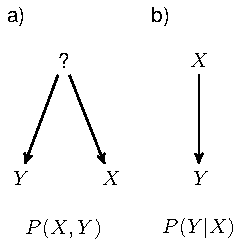
\includegraphics[scale=0.9,right]{fig-fst.pdf}
\end{columns}
\end{frame} %-------------------------------------------------------------------

\begin{frame}{Aim 1 - Evolution FST} %------------------------------------------
% Evolution FST
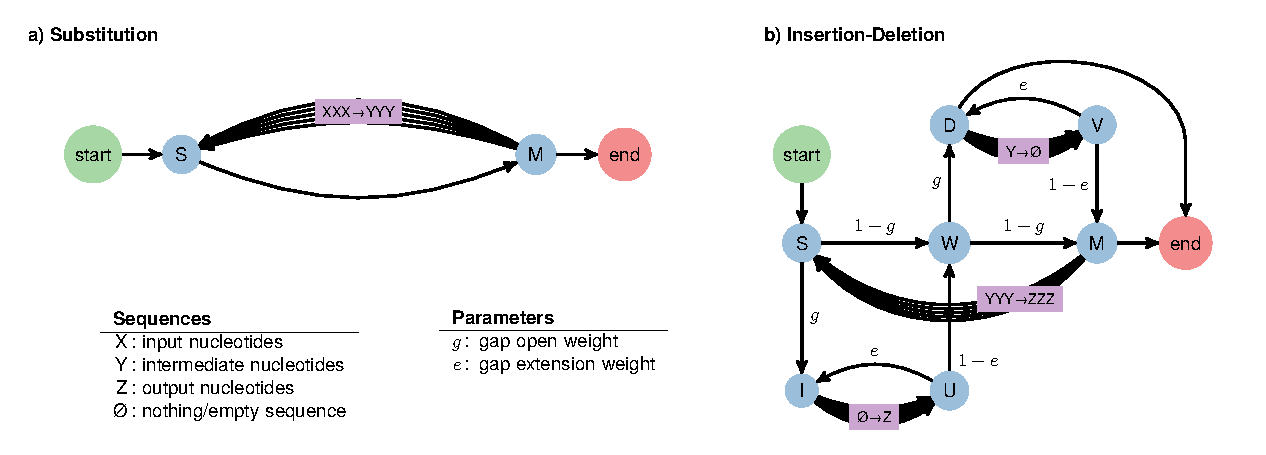
\includegraphics[scale=0.6,center]{fig-evolution-fst.pdf}
\begin{itemize}
	\item Composing (a) and (b) results in the evolution FST.
	\item Each state node represents a state in an FST.
	\item Arcs display possible transitions and their weights.
\end{itemize}
\note[item]{(a) encodes a 64x64 codon substitution matrix}
\note[item]{(b) models insertions and deletions}
\end{frame} %-------------------------------------------------------------------

\begin{frame}{Aim 1 - Substitution Model} %-------------------------------------
Codon substitution with instantaneous substitution rate matrix $Q$:
\vspace{1em}
\begin{align*} Q_{ij} &= \begin{cases}
    \mu_{ij} & \text{if $i$ and $j$ are synonymous}\\
    \omega \cdot \mu_{ij} & \text{if $i$ and $j$ are nonsynonymous}
    \end{cases}\\[10pt]
   Q_{ii} &= -\sum_{j:j \neq i} Q_{ij}
\end{align*}
\begin{itemize}
	\item $\mu_{ij}$: mutation rate of codon $i$ to $j$.
	\item $\omega$: coefficient of selection.
	\item Supports a variety of models (e.g.
		MG94\parencite{muse_gaut_1994}, ECM\parencite{kosiol_ECM_2007}).
	% \item $t$: evolutionary time.
	% \item $P(j | i;t) = {\rm e}^{Qt}$.
\end{itemize}
\note[item]{Muse \& Gaut 1994, describe}
\note[item]{Empirical Codon Model, describe}
\end{frame} %-------------------------------------------------------------------

\begin{frame}{Aim 1 - Dynamic Programming} %------------------------------------
\vspace{1em}
\begin{itemize}
	\item FST pairwise alignment is performed via \textbf{composition}
		(expensive).
	\item Solution: reducing the evolution FST to three states and aligning via
		dynamic programming.
\end{itemize}
\vspace{-0.75em}
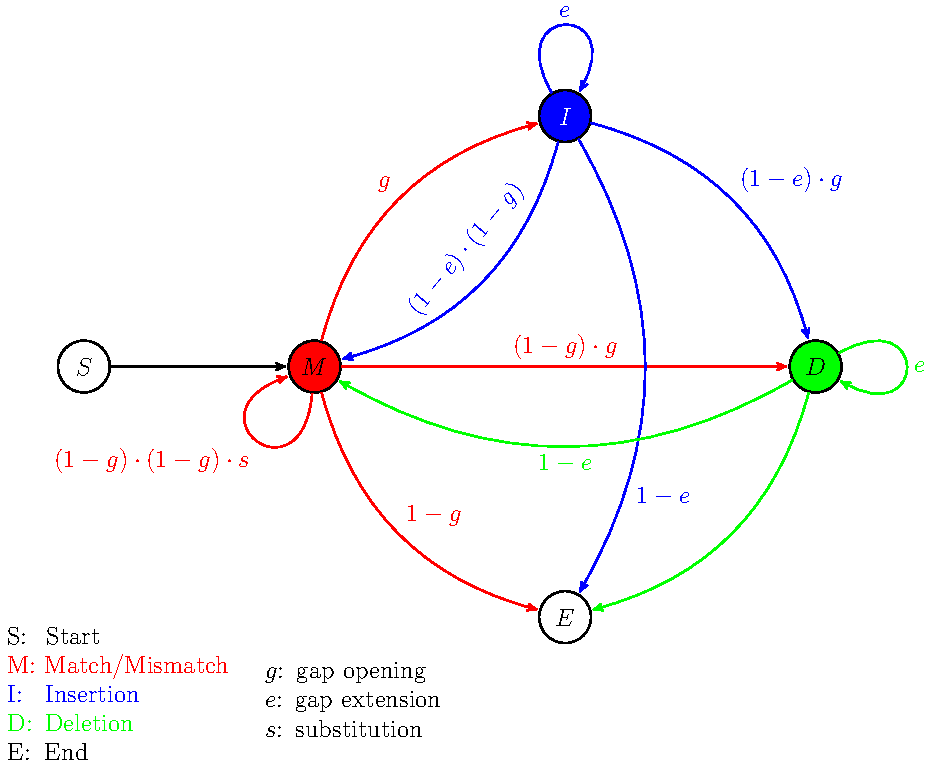
\includegraphics[scale=0.5,center]{fig-dp-model.pdf}
\note[item]{which is a powerful operation that allows complex FSTs to be build
	from smaller parts. However, composition can be prohibitive when aligning
	sequence of a few thousand nucleotides and up. To solve this issue, the
	FST can be reduced to three states and solved via dynamic programming.}
\end{frame} %-------------------------------------------------------------------

\begin{frame}{Aim 2 - Artifacts} %------------------
% Artifacts \& heterogeneous approach (high and low qual sequences)
\justify
\begin{itemize}
	\setlength\itemsep{1em}
	\item Artifacts are common in genomic data sets, especially in non-model
		organisms.
	\item Current practices involve discarding data.
	\item COATi will align a sequence from a non-model organism against a
		high-quality sequence as a path through an FST.
\end{itemize}
\end{frame} %-------------------------------------------------------------------

\begin{frame}{Aim 2 - Marginal Substitution Model} %----------------------------
\begin{itemize}
	\setlength\itemsep{1em}
	\item Substitution models assume sequences are accurate.
	\item Not the case for non-reference genomes.
	\item Solution: pairwise align a high-quality against a low-quality sequence.
	\item Marginal substitution model is robust to erroneous nucleotides.
\end{itemize}
\vspace{2em}

\[P'_{cod_1,nuc,pos} = \mathlarger{\mathlarger{\sum}}_{cod_2} \thickspace \begin{cases}
	P(cod_1 \thinspace | \thinspace cod_2) \enspace \text{if} \enspace cod_{pos} = nuc\\
	0 \enspace \text{otherwise}
\end{cases} \]

% \begin{itemize}
% 	\item $\sum_{cod_2}$: sum over all 64 codons.
% 	\item $P(cod_1 \thinspace | \thinspace cod_2)$: 64x64 codon substitution matrix.
% 	\item $cod_{pos} = nuc$: true if nucleotide in $cod_1[pos]$ is equal to $nuc$.
% \end{itemize}
\note[item]{From 64x64 (MG94/ECM) to 64x4x3}
\end{frame} %-------------------------------------------------------------------

\begin{frame}{Aim 2 - Ambiguous Data} %-----------------------------------------
\begin{columns}
\column{0.6\textwidth}	
\begin{itemize}
	\setlength\itemsep{1em}
	\item Ambiguous nucleotides are common in low-quality data.
	\item Marginal model will handle all 15 cases for descendant sequence.
	\item Typically replaced by average over all possibilities.
	\item Alternative approaches to handle ambiguous data.
\end{itemize}
\column{0.4\textwidth}	
\includegraphics[width=0.9\textwidth]{images/iupac.png}
\end{columns}
\footnotetext{https://www.bioinformatics.org/sms/iupac.html}
\note[item]{Best nucleotide. Maybe as a function of $t$ (weighted avg;
	smaller $t$ => more weight to best, larger $t$ => more avg)?}
\end{frame} %-------------------------------------------------------------------

\begin{frame}{Aim 2 - Model Frameshifts} %--------------------------------------
\begin{columns}
\column{0.5\textwidth}	
\begin{itemize}
	\setlength\itemsep{1em}
	\item FST that specifically models frameshifts (lengths 1-2).
	\item Longer frameshifts are modeled by setting the indel FST to length
		multiple of 3 and composing with the frameshift FST.
	% \item Compare approaches
\end{itemize}
\column{0.5\textwidth}	
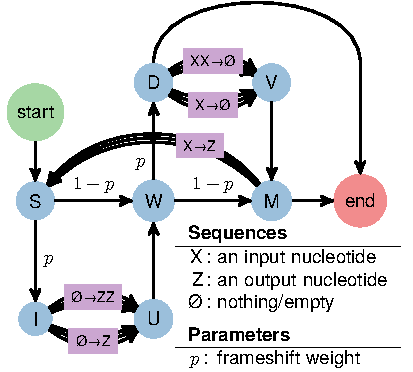
\includegraphics[width=0.9\textwidth]{fig-fst-frameshifts.pdf}
\end{columns}
\note[item]{Compare approaches}
\end{frame} %-------------------------------------------------------------------

\begin{frame}{Aim 2 - Biological Frameshifts} %---------------------------------
\begin{itemize}
	\setlength\itemsep{1em}
	\item Frameshifts in coding sequences are expected to be artifacts due to
		purifying selection.
	\item In some cases frameshifts are believed to be biological.
	\item To my knowledge, this particular issue has not been addressed.
\end{itemize}
\note[item]{Cases: pairs of compensatory indels, frameshifts in
	\textit{Saccharomyces cerevisiae} (collaborators; "un-studied").}
\note[item]{Not addressed the problem yet; ideas: convert to DNA after frameshift,
	"correct" reading frame after frameshift.}
% Committee will ask how do I plan on addressing this!
% What cases? Pairs of compensatory indels? 

\end{frame} %-------------------------------------------------------------------

\begin{frame}{Aim 3 - Expectation-Maximization} %-------------------------------
\begin{itemize}
	\setlength\itemsep{1em}
	\item Ability to infer parameters estimates from data.
	\item EM \parencite{dempster_laird_rubin_EM_1977} is a classic iterative
		method for deriving estimates of parameters in statistical models with
		latent variables.
	\item E-step: infer information about latent variables.
	\item M-step: improve parameter estimates.
\end{itemize}
\end{frame} %-------------------------------------------------------------------

\begin{frame}{Aim 3 - Parameters} %---------------------------------------------
% Substitution and indel model parameters
\textbf{Substitution model}
\begin{itemize}
	\item GTR\parencite{tavare_gtr_1986} underlying model for MG94:
		6 nucleotide transition $\bm{\sigma}$.
	\item 4 nucleotide or 64 codon frequencies: $\bm{\pi}$.
	\item Coefficient of selection $\bm{\omega}$.
\end{itemize}

\vspace{2em}
\textbf{Indel model}
\begin{columns}[T]
\column{0.5\textwidth}	
Standard model
\begin{itemize}
	\item Gap opening: $\bm{g}$.
	\item Gap extension: $\bm{e}$.
\end{itemize}
\column{0.5\textwidth}	
Extended model
\begin{itemize}
	\item Insertion opening: $\bm{i_o}$.
	\item Insertion extension: $\bm{i_e}$.
	\item Deletion opening: $\bm{d_o}$.
	\item Deletion extension: $\bm{d_e}$.
\end{itemize}
\end{columns}
\end{frame} %-------------------------------------------------------------------

% \begin{frame}{Aim 3} %----------------------------------------------------------
% Validation?
% \end{frame} %-------------------------------------------------------------------

% \begin{frame}{Preliminary Data} %-----------------------------------------------
% Summarize what's been done
% \end{frame} %-------------------------------------------------------------------

\begin{frame}{Preliminary Data} %-----------------------------------------------
\begin{itemize}
	\item Downloaded 4000 human-gorilla homologous pairs from ENSEMBL
		\parencite{ensembl_hubbard_2002}.
	\item Aligned and extracted gap patterns from 1660 sequences.
	\item Introduced gaps into remaining 2340 sequences to simulate `true' data set.
	\item Remove gaps and compare accuracy of aligners retrieving `true' data.
	{\setlength\itemindent{15pt} \item[ ] Distance metric}
	{\setlength\itemindent{15pt} \item[ ] Number of perfect alignments}
	{\setlength\itemindent{15pt} \item[ ] Accuracy of selection}

\end{itemize}
\end{frame} %-------------------------------------------------------------------

\begin{frame}{Preliminary Data} %-----------------------------------------------
\resizebox{1.03\linewidth}{!}{% Resize table to fit within \linewidth horizontally
\hspace{-0.8em}\centering{% \begin{table}[h!]
% \begin{adjustbox}{width=\columnwidth,center}
\definecolor{asublue}{RGB}{0,163,224}

\begingroup\centering
\begin{tabular}{r|ccccc}
      & \textbf{COATi} & \textbf{PRANK} & \textbf{MAFFT} & \textbf{CLUSTAL$\Omega$} & \textbf{MACSE}\\
\hline
Avg alignment error ($d_{seq}$) & \cellcolor{asublue!25}0.00060 & 0.01086 & 0.00671 & 0.01300 & 0.00611\\
Perfect alignments & \cellcolor{asublue!25}1300 & 86 & 1282 & 634 & 1059\\
Best alignments & \cellcolor{asublue!25}1756 & 188 & 1463 & 666 & 1129\\
Imperfect alignments & \cellcolor{asublue!25}437 & 1651 & 455 & 1109 & 678\\
% \hline
Accuracy of positive selection & \cellcolor{asublue!25}97.3\pct & 87.3\pct & 85.8\pct & 69.1\pct & 81.5\pct\\
Accuracy of negative selection & \cellcolor{asublue!25}99.8\pct & 98.9\pct & 98.7\pct & 97.3\pct & 98.5\pct
\end{tabular}
\par\endgroup
% \end{adjustbox}
% \end{table}

% NEWEST comparison data 2022/06/09, inferring gaps from all 5 methods
% mcoati	0.00059 9270130816151
% prank		0.01086 33839725945
% mafft		0.00670 545158536942
% clustalo	0.01299 61253293471
% macse		0.00611 069632339777
% [1] "Perfect alignments"
%   mcoati    prank    mafft clustalo    macse
%     1300       86     1282      634     1059
% [1] "Best alignments"
% [1] 1756  188 1463  666 1129
% [1] "Imperfect alignments"
% [1]  437 1651  455 1103  678
% [1] "Species gorilla with model mcoati"
% [1] "ka root mean-squared error:0.000461080945838058"
% [1] "ks root mean-squared error:0.000935195768612048"
% [1] "Accuracy of + selection:0.973404255319149"
% [1] "Accuracy of - selection:0.99767549976755"
% [1] "Species gorilla with model prank"
% [1] "ka root mean-squared error:0.0428559577365695"
% [1] "ks root mean-squared error:0.225105734336453"
% [1] "Accuracy of + selection:0.87292817679558"
% [1] "Accuracy of - selection:0.989287377736376"
% [1] "Species gorilla with model mafft"
% [1] "ka root mean-squared error:0.0307718945528414"
% [1] "ks root mean-squared error:0.039579523100722"
% [1] "Accuracy of + selection:0.857881136950904"
% [1] "Accuracy of - selection:0.987182474947565"
% [1] "Species gorilla with model clustalo"
% [1] "ka root mean-squared error:0.0490336010168609"
% [1] "ks root mean-squared error:0.0641562105407489"
% [1] "Accuracy of + selection:0.691292875989446"
% [1] "Accuracy of - selection:0.972784368457781"
% [1] "Species gorilla with model macse"
% [1] "ka root mean-squared error:0.0241886043324206"
% [1] "ks root mean-squared error:0.0544004979209871"
% [1] "Accuracy of + selection:0.81524926686217"
% [1] "Accuracy of - selection:0.985473829836292"
}
}
\vspace{1em}
\begin{itemize}
	\item COATi performs best on all metrics.
	\item AA-based aligners (CLUSTAL$\Omega$, MACSE) have difficulties retrieving
		positive selection.
	\item Aligners that don't allow frameshifts (PRANK, CLUSTAL$\Omega$) have the
		highest alignment error.
	\item Tools that model frameshifts (MAFFT, MACSE) lower aln error but also
		have difficulties with positive selection.
\end{itemize}
% Pinpoint shortcomings of aligners
\note[item]{1st row: distance metric, the lower the better.}
\note[item]{Clustal$\Omega$ has difficulty "recovering/maintaining" positive
selection given its AA-based alignment.}
\end{frame} %-------------------------------------------------------------------

\begin{frame}{Preliminary Data - Memory and Runtime} %--------------------------
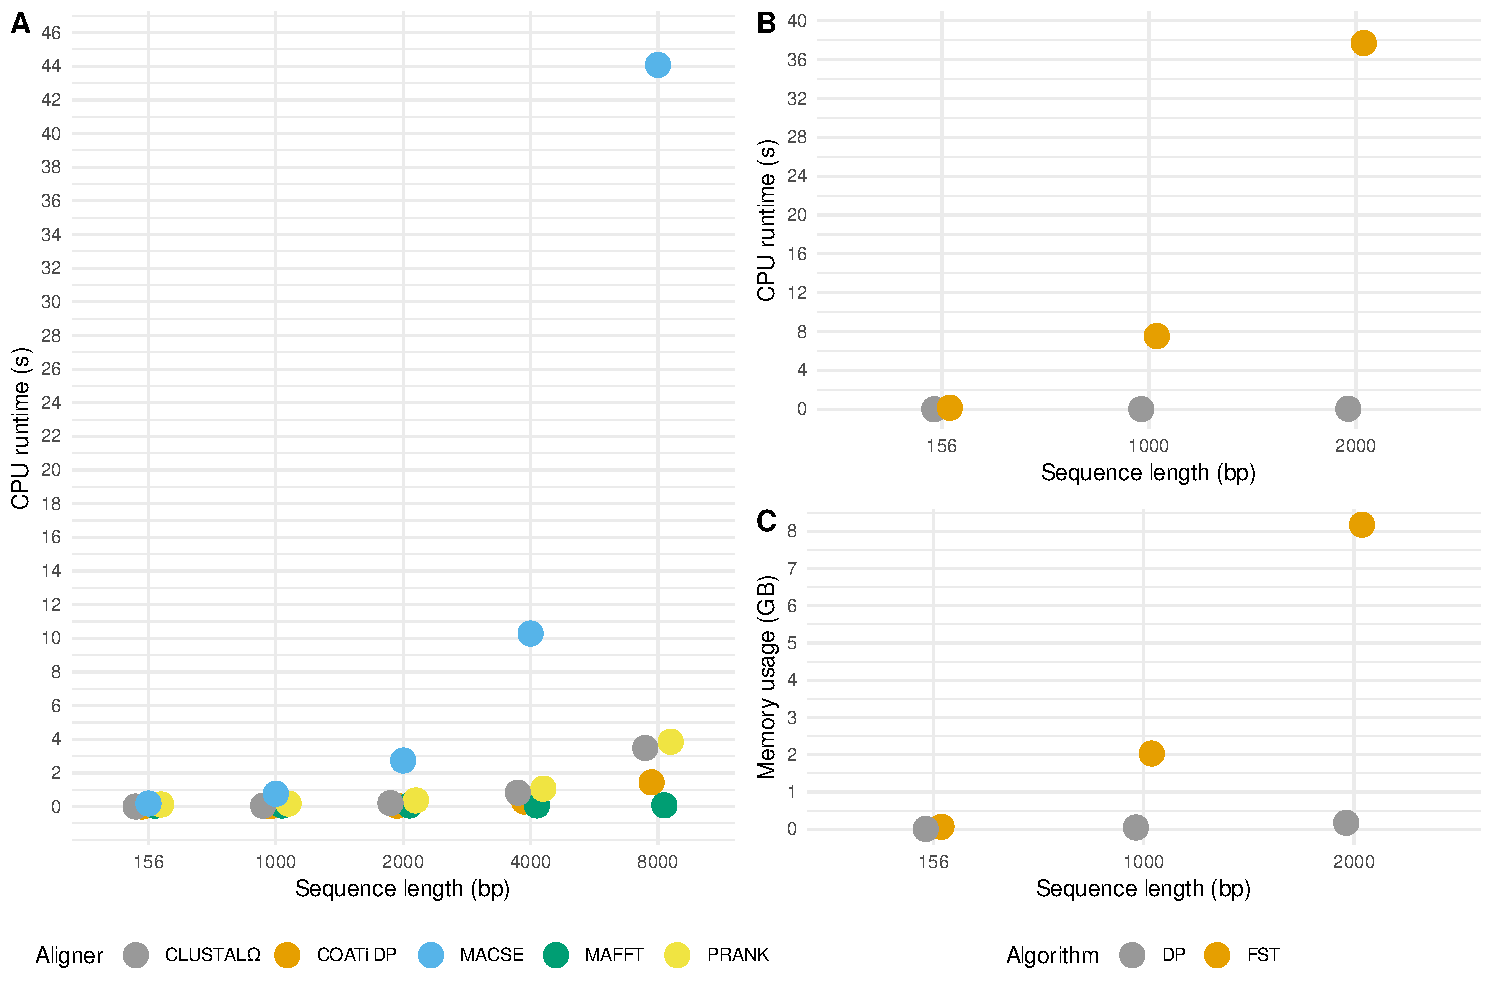
\includegraphics[scale=0.45,center]{fig-benchmark.pdf}
\end{frame} %-------------------------------------------------------------------

\begin{frame}{Future work} %----------------------------------------------------
Extend COATi pairwise to multiple sequence alignment.
\vspace{1em}
\begin{itemize}
	\setlength\itemsep{1em}
	\item Initial alignment without an input phylogenetic tree.
	\item Iterative refinement by sampling alignment space.
\end{itemize}
\end{frame} %-------------------------------------------------------------------

\begin{frame}{Questions} %------------------------------------------------------
\includegraphics[scale=0.1,center]{images/lab.jpg}
\end{frame} %-------------------------------------------------------------------

% ##############################################################################
\appendix %#####################################################################

\begin{frame}[t,allowframebreaks]{References} %---------------------------------
\printbibliography
\end{frame} %-------------------------------------------------------------------


% ##############################################################################
\appendix % ####################################################################
% Supplemental slides

\begin{frame}[noframenumbering]{Distance Metric} %------------------------------
\begin{columns}
\column{0.5\textwidth}
Non-negative function, $d(x,y)$, metric conditions:
\begin{itemize}
	\item $d(x,y) = 0$ iff $x=y$
	\item $d(x,y) = d(y,x)$ symmetry
	\item $d(x,z) \leq d(x,y) + d(y,z)$ triangle inequality
\end{itemize}
\column{0.5\textwidth}
\includegraphics[scale=0.15,center]{/fig-sop-problems.png}
\end{columns}
\footnotetext[1]{\cite{metrics_blackburne_whelan_2011}}
\note[item]{For a function to be a valid metric has to meet all three criteria
	(explain briefly). Sum of pairs, a common score used to evaluate differences
	between MSA based on the number of matches on each column, has been proven
	to not satisfy all 3 conditions. An example (fig).}
\end{frame} %-------------------------------------------------------------------

\begin{frame}[noframenumbering]{Distance Metric} %------------------------------
\includegraphics[scale=0.25,center]{fig-distance-metrics.png}

\vspace{1em}
\begin{align*}
d(A,B) = \frac{1}{c} \sum_i \sum_j d(A,B)^i_j = \frac{1}{c} \sum_i \sum_j \frac{|H(A)^i_j \triangle H(B)^i_j|}{|H(A)^i_j|+|H(B)^i_j|}
\end{align*}

\footnotetext[1]{\cite{metrics_blackburne_whelan_2011}}
\note[item]{Homology set: characters on the same column, i.e. nucleotides said to
	be homologous.}
\note[item]{Hamming distance: number of different positions or minimum number of
	substitutions required to change one set into the other.}
\end{frame} %-------------------------------------------------------------------

\begin{frame}[noframenumbering] %-----------------------------------------------
\centering{\resizebox{0.85\linewidth}{!}{% Resize table to fit within \linewidth horizontally
\input{../resources/figures/table-example-dseq.tex}
}}

\vspace{1em}
\begin{columns}
\column{0.5\textwidth}
$d_seq(A,B)^1_1=0$ \\
$d_seq(A,B)^2_1=0$ \\
$d_seq(A,B)^3_1=0$ \\
\column{0.5\textwidth}
$d_seq(A,B)^1_2=\frac{2}{4}=\frac{1}{2}$ \\
$d_seq(A,B)^2_2=\frac{1}{4}$ \\
$d_seq(A,B)^3_2=\frac{1}{4}$ \\
\end{columns}
\end{frame} %-------------------------------------------------------------------

\begin{frame}[noframenumbering]{Accuracy of Selection} %------------------------
$d_N$ and $d_S$ ($d_N/d_S = \omega$) are used to estimate the selection a given protein or DNA
section is experiencing.

\vspace{1em}
\begin{itemize}
	\item $d_N$: number of non-synonymous changes over non-synonymous sites.
	\item $d_S$: number of synonymous changes over synonymous sites.
	\item $\omega \approx 1$: neutral selection.
	\item $\omega > 1$: positive selection.
	\item $\omega < 1$: purifying selection.
\end{itemize}
\end{frame} %-------------------------------------------------------------------

\begin{frame}[noframenumbering]{Accuracy of Selection} %------------------------
$F_1$ score to test correct inference of selection.

\begin{align*}
F_1 &= \left( \frac{2}{recall^{-1} + precision^{-1}} \right)\\
	&= 2 \cdot \frac{precision \cdot recall}{precision + recall}\\
	&= \frac{2 \cdot TP}{2 \cdot TP+FP+FN}
\end{align*}

\vspace{1em}
Where precision$=\frac{TP}{TP+FP}$ and recall$=\frac{TP}{TP+FN}$.
\note[item]{$F_1$: weighted average of precision and recall. More informative score
	/statistic than accuracy.}
\note[item]{Precision: ratio of correctly predicted positive observations to total
	predicted pos obs. Recall: (sensitivity) ratio of correctly predicted pos obs
	to all obs true positives.}
\note[item]{sensitivity=TP/(TP+FN); specificity=TN/(TN+FP); precision=TP/(TP+FP);
	accuracy=(TP+TN)/(TP+FN+TN+FP)}
\end{frame} %-------------------------------------------------------------------

% \begin{frame}{Aim 3} %----------------------------------------------------------
% Validation?
% \end{frame} %-------------------------------------------------------------------

% Add slide comparing initial methods (coati-fst, coati-dna, coati-marg, ecm?)
% % software comparison coati_dna coati_toy coati_marg ecm ecm_marg PRANK MAFFT ClustalO \Omega
% % 354 sequences
%
% \centering \textbf{Gorilla - human comparison (1334 alignments)}
%
% \begin{table}[h!]
% \begin{adjustwidth}{-4.7cm}{}
% \begin{tabular}{r|ccccccccc}
%       & \textbf{coati} & \textbf{marg} & \textbf{dp\_marg} & \textbf{dna} & \textbf{ecm} & \textbf{ecm\_marg} & \textbf{PRANK} & \textbf{MAFFT} & \textbf{Clustal $\Omega$} \\
% \hline
% Avg alignment error ($d_{seq}$) & 0.000901 & 0.000909 & \colorbox{blue!25}{0.000897} & 0.000910 & 0.000927 & 0.000915 & 0.005319 & 0.009414 & 0.013290\\
% %Average alignment error ($d_{pos}$) & 0.01538 & 0.01546 & \colorbox[HTML]{00A3E0}0.01512 & - & 0.03298 & 0.02751 & 0.03645\\
% Perfect alignments & 962 & 938 & \colorbox{blue!25}{971} & 951 & 958 & 949 & 18 & 865 & 695\\
% Best alignments & 1093 & 1069 & \colorbox{blue!25}{1108} & 1088 & 1083 & 1078 & 42 & 887 & 704\\
% Imperfect alignments & 147 & 171 & \colorbox{blue!25}{138} & 158 & 151 & 160 & 1091 & 244 & 414\\
% \hline
% $k_a$ root mean-squared error & 0.00049 & 0.00049 & 0.00048 & 0.00054 & 0.00068 & \colorbox{blue!25}{0.00039} & 0.00838 & 0.04351 & 0.05520\\
% $k_s$ root mean-squared error & 0.00099 & 0.00100 & 0.00097 & \colorbox{blue!25}{0.00095} & 0.00137 & 0.00107 & 0.01800 & 0.05235 & 0.06827\\
% Positive selection F1 score & 98.7\pct & 98.7\pct & 98.7\pct & 98.3\pct & \colorbox{blue!25}{99\pct} & \colorbox{blue!25}{99\pct} & 19.7\pct & 83.2\pct & 77.3\pct \\
% Negative selection F1 score & 99.8\pct & 99.8\pct & 99.8\pct & 99.8\pct & \colorbox{blue!25}{99.9\pct} & \colorbox{blue!25}{99.9\pct} & 90.1\pct & 97.9\pct & 97.1\pct \\
% \end{tabular}
% \end{adjustwidth}
% \end{table}
%
% \vspace{1cm}
%
% \centering \textbf{\textit{C. jacchus} - human comparison (1137 alignments)}
%
% \begin{table}[h!]
% \begin{adjustwidth}{-4cm}{}
% \begin{tabular}{r|ccccccccc}
%       & \textbf{dna} & \textbf{toy} & \textbf{marg} & \textbf{ecm} & \textbf{ecm\_marg} & \textbf{PRANK} & \textbf{MAFFT} & \textbf{Clustal $\Omega$} \\
% \hline
% Avg alignment error ($d_{seq}$) & 0.00202 & \colorbox{blue!25}{0.00195} & \colorbox{blue!25}{0.00195} & 0.00242 & 0.00393 & 0.00779 & 0.01501 & 0.01990\\
% %Average alignment error ($d_{pos}$) & \celcollor{asublue!25}0.01885 & 0.01889 & 0.01904 & - & 0.03588 & 0.03113 & 0.03930\\
% Perfect alignments & 574 & \colorbox{blue!25}{582} & 581 & 512 & 166 & 15 & 444 & 221\\
% Best alignments & 830 & 829 & \colorbox{blue!25}{841} & 728 & 247 & 50 & 506 & 241\\
% Imperfect alignments & 155 & \colorbox{blue!25}{147} & 148 & 217 & 563 & 712 & 285 & 508\\
% \hline
% $k_a$ root mean-squared error & 0.00136 & \colorbox{blue!25}{0.00131} & 0.00135 & 0.00241 & 0.00360 & 0.01760 & 0.05287 & 0.06277\\
% $k_s$ root mean-squared error & 0.00402 & 0.00359 & \colorbox{blue!25}{0.00358} & 0.00449 & 0.01070 & 0.03917 & 0.06598 & 0.08086\\
% Positive selection F1 score & \colorbox{blue!25}{88.9\pct} & \colorbox{blue!25}{88.9\pct} & \colorbox{blue!25}{88.9\pct} & 82.4\pct & NA & 77.8\pct & 60\pct & 66.7\pct \\
% Negative selection F1 score & 99.9\pct & 99.9\pct & 99.9\pct & 99.9\pct & \colorbox{blue!25}{100\pct} & 99.8\pct & 99.6\pct & 99.7\pct \\
% \end{tabular}
% \end{adjustwidth}
% \end{table}
% \vspace{1cm}
%
% \centering \textbf{Mouse - human comparison (354 alignments)}
%
% \begin{table}[h!]
% \begin{adjustwidth}{-4cm}{}
% \begin{tabular}{r|cccccccc}
%       & \textbf{dna} & \textbf{toy} & \textbf{marg} & \textbf{ecm} & \textbf{ecm\_marg} & \textbf{PRANK} & \textbf{MAFFT} & \textbf{Clustal $\Omega$} \\
% \hline
% Avg alignment error ($d_{seq}$) & 0.00991 & 0.00870 & \colorbox{blue!25}{0.00865} & 0.00893 & 0.01423 & 0.02835 & 0.04075 & 0.04494 \\
% %Average alignment error ($d_{pos}$) & 0.03345 & \colorbox{blue!25}{0.03123} & 0.03130 & - & 0.05074 & 0.04731 & 0.05229\\
% Perfect alignments & 47 & 52 & \colorbox{blue!25}{53} & 44 & 10 & 0 & 36 & 17\\
% Best alignments & 164 & 209 & \colorbox{blue!25}{218} & 178 & 39 & 3 & 46 & 23\\
% Imperfect alignments & 18 & 13 & \colorbox{blue!25}{12} & 21 & 55 & 65 & 29 & 48\\
% \hline
% $k_a$ root mean-squared error & 0.00317 & 0.00268 & \colorbox{blue!25}{0.00260} & 0.00385 & 0.00455 & 0.06711 & 0.10787 & 0.12277\\
% $k_s$ root mean-squared error & 0.03708 & 0.03012 & 0.02988 & \colorbox{blue!25}{0.02590} & 0.48282 & 0.53374 & 0.13212 & 0.17016\\
% Positive selection F1 score & NA & NA & NA & NA & NA & NA & NA & NA \\
% Negative selection F1 score & \colorbox{blue!25}{100\pct} & \colorbox{blue!25}{100\pct} & \colorbox{blue!25}{100\pct} & \colorbox{blue!25}{100\pct} & \colorbox{blue!25}{100\pct} & \colorbox{blue!25}{100\pct} & 99.86\pct & \colorbox{blue!25}{100\pct} \\
% \end{tabular}
% \end{adjustwidth}
% \end{table}

\end{document}

% \begin{frame}{Sequence Alignment} %---------------------------------------------
% % \includegraphics[scale=0.15,center]{figures/fig-mafft.png}
% \begin{itemize}
% \item Hypothesis of which characters from two or more sequences are related by
% 	common descent \parencite{problems_cartwright_2009}.
% \vspace{1em}
% \item Cornerstone for analyses in comparative and functional genomics.
% \end{itemize}
% \footnotetext[1]{\cite{mafft_katoh_2009}}
% \note[item]{Sequence alignment can be seen as the hypothesis of which characters
% 	from two or more sequences are homologous/related by common descent. A MSA
% 	is the base for multiple analyses in comparative and functional genomics and
% 	phylogenetics.}
% \note[item]{This shows a typical procedure (progressive aln) on how to compose MSA
%  	(MAFFT). Start with raw unaligned sequences, compute all pairwise alignments,
% 	construct distance matrix and generate a tree to guide the group-to-group alignments.
% 	This can be iterated until convergence.}
% \end{frame} %-------------------------------------------------------------------

